Software translations are the intrinsic idea of compilers where source code written in a (domain-specific) programming language is translated into formulations of a mostly more low-level intermediate or directly machine-readable language \cite{Aho:1986:CPT:6448,Stanier:2013:IRI:2480741.2480743}.
Software translations are also demanded in scenarios where programs written in a diverse set of programming languages may be translated into a unified language for unified maintainability and verification \cite{DBLP:conf/icmt/0001GNEBMPEE14}.
Apart from such text-to-text translations, a much older tradition is to translate textual representations into visual models which reflect the cognitive concepts we had in mind when preparing and writing the texts from different domains (text-to-model translations) \cite{striewe_08_using} and vice versa (model-to-text translations) \cite{jsc12}.
In the software world this trend was enforced by model-driven engineering (MDE) approaches \cite{6507223} where source code is represented by diagram models in a diverse set of different domain specific visual modelling languages (e.g. UML) and vice versa source code is generated from models not only in the development phase but also for maintenance after the systems have been deployed (cf. \cref{fig:sec-compl-software-trans:software_trans_types}).

We do not concentrate on the reasons for translations (e.g., reducing or creating abstractions) but on the well-known formal concept of graph grammars \cite{Ehrig:2006:FAG:1121741} from \cref{sec-gt-trafo} as a generalisation of word grammars for specifying model transformations \cite{FAGT2,Mens2006125,118} in general (cf. \cref{sec-mt-tgg}) and text-to-text \cite{DBLP:conf/staf/0001NBEG14} as well as text-to-model (model-to-text) translations in particular.
In the context of graph grammars, models are represented by graphs whereas the translation of models is specified by a graph grammar, i.e., a set of graph transformation rules together with a start graph.
This allows the verification of the completeness of translations.
A translation from language $\Lang_1$ to $\Lang_2$ is syntactically complete, if all elements of $\Lang_1$ can be completely translated.
The completeness problem can be reformulated as a language inclusion problem $\Lang_1 \subseteq \Lang_3$ where $\Lang_3$ is the language induced by the given graph grammar which specifies the translation (cf. \cref{sec-compl-software-trans-completeness,fact:comp_soft_trans}).
In general, the language inclusion problem is undecidable for context-free grammars $\Lang_3$, most of their sub-classes and all classes above \cite{Asveld2000247} (cf. \cref{sec-dc-general}).
Therefore, we developed sufficient conditions (called domain completeness \cite{DBLP:conf/staf/Nachtigall0BE14}) to approximately solve the inclusion problem for languages $\Lang_1$ that are given by a type graph \cite{DBLP:journals/tcs/GolasLEO12} together with a set of graph constraints \cite{DBLP:conf/birthday/HabelP05,FAGT2} and languages $\Lang_3$ that are given by a graph grammar (cf. \cref{sec-dc-verification,sec-dom-compl-mt}).
We concentrate on instantiating the general concept of domain completeness of model transformations from \cref{sec-dom-compl-mt} to the completeness problem of software translations in \cref{sec-compl-software-trans-prob} by closing the gap between the definition of programming languages and the definition of graph languages in \cref{sec-compl-software-trans-mapping}.
Derivation trees of context-free grammars are represented by typed attributed graphs \cite{DBLP:journals/tcs/GolasLEO12} with a tree-structure.
Therefore, we present an encoding of context-free word grammars to attributed type graphs together with graph constraints such that the language of derivation trees that is induced by the word grammar is isomorphic to the graph language that is induced by the type graph together with the graph constraints (cf. \cref{sec-compl-software-trans-mapping,thm:sec-compl-software-trans:equ_lang_der}).
This allows the application of the domain completeness verification from \cref{sec-dom-compl-mt} in the graph transformation world in order to check if all abstract syntax trees that can be formed over a programming language can actually be translated. 
For unambiguous programming languages $L$ \cite{DBLP:books/daglib/0011126} that have a unique derivation tree for each program, this gives a good hint towards the syntactical completeness of the translation of programs written in $L$.

\begin{figure}[!tb]
\begin{center}
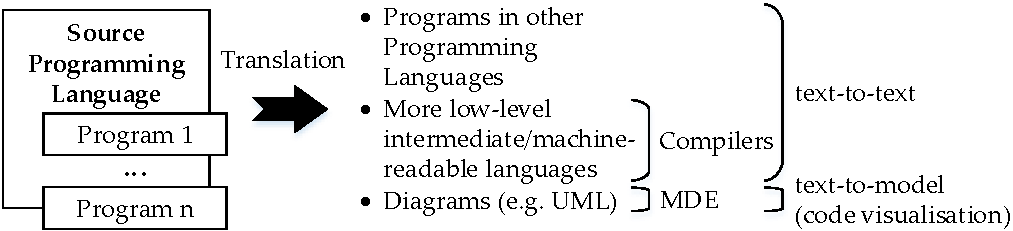
\includegraphics[width=.85\textwidth]{img/software_trans/software_trans2.pdf}
\end{center}
\caption{Types of Software Translations}
\label{fig:sec-compl-software-trans:software_trans_types}
\end{figure}
